    \section{Introduction}
\label{sec:intro}

Segmenting images is a core problem in Computer Vision, yet achieving high-quality results typically requires extensive human effort to annotate pixel-level masks. Moreover, conventional semantic segmentation methods ~\cite{chen2017deeplab, he2017mask, kirillov2018panoptic, cheng2022masked} struggle to generalize to unseen categories. Inspired by the human ability to recognize novel objects from just a few examples, few-shot segmentation (FSS) \cite{li2021adaptive, wang2019panet, liu2022learning,  shaban2017one} has emerged as a paradigm that leverages a small set of labeled reference samples to guide the segmentation of target images containing arbitrary, previously unseen classes.

To this end, recent work has turned to visual foundation models (VFMs) \cite{bommasani2021opportunities}, which offer rich visual representations and strong generalization capabilities \cite{radford2021clip, yuan2023power}. A natural approach \cite{liu2023matcher, zhang2024bridge, sun2024vrp} is to decouple the few-shot segmentation task into two stages: feature matching followed by promptable segmentation. This is typically achieved by combining DINOv2 \cite{oquab2023dinov2}, known for its strong semantic correspondence capabilities \cite{zhang2023tale, meng2024segic, zhang2024telling, tang2023emergent}, with Segment Anything  \cite{kirillov2023segment}, which excels at producing high-quality segmentation masks \cite{kirillov2023segment, zou2023segment, zhang2023personalize}. While effective,
these modular approaches add computational overhead and require prompt engineering to coordinate multiple VFMs \cite{zhu2024unleashing}. 

We observe that Segment Anything 2 (SAM2) \cite{ravi2024sam} offers an alternative paradigm.
Designed for Video Object Segmentation, it operates as a \textit{prompt-and-propagate} framework, where an object is specified via its mask and tracked across frames. 
To achieve this, \sam{} introduces a \texttt{Memory Attention} mechanism to implicitly match features across video frames and propagate masks over time with high spatial precision. While this feature matching is originally intended for object tracking based on visual similarity, we note that this architecture inherently unifies two capabilities central to FSS \textit{within a single model}: dense feature matching and high-quality mask generation. Building on this analogy, we propose repurposing the \textit{prompt-and-propagate} framework to address the FSS task, by reinterpreting the temporal dimension of videos as a collection of semantically related images.



This raises the central question: \textit{instead of limiting \sam{} to \textbf{object tracking}, can it generalize beyond visual similarity to perform \textbf{semantic tracking} based on shared concepts across images}? 

Addressing this inquiry means, in turn, to answer whether SAM2
has implicitly learned semantic-aware representations, despite its class agnostic pre-training. To answer this, we conduct a toy experiment in \cref{fig:isic}, testing \sam{} performance on FSS datasets with different semantic variability. Interestingly, we observe that in low-semantic-shift scenarios, \sam{} achieves comparable or even higher performance with respect to state-of-the-art methods. However, on challenging datasets with high semantic shift, its performance drops drastically. 
A straightforward conclusion from
these preliminary results would be that \sam{} may not have learned discriminative representations in its class-agnostic pretraining, making it unsuited for tasks requiring semantic alignment.

We challenge this interpretation, based on the observation that \sam{} pretraining, focused on instance matching across frames, shares similarities with self-supervised learning frameworks \cite{yang2022inscon, yang2021instance, henaff2021efficient, bardes2022vicregl}, which are known to elicit semantic understanding by enforcing feature invariance across views \cite{caron2021emerging, bardes2021vicreg}.
Given this analogy, we posit that SAM2 \emph{does} encode semantic information, which is however entangled with instance-specific features optimized for object tracking, reflecting experimental evidence in \cref{fig:isic}. If our intuition is true, it implies that \textit{i)} this structure could be disentangled through lightweight transformations \cite{aghajanyan2020intrinsic, hu2022lora, li2018measuring}, such as adapter modules and \textit{ii)} it should be learnable from a set of base classes and generalize to unseen categories \cite{rusu2018meta, cheng2023meta}. 
To this end, we \textit{i)} intentionally use one of the simplest adapters in the literature, namely AdaptFormer \cite{houlsby2019adapter}, and \textit{ii)} verify the generalization hypothesis through extensive experiments in strict few-shot benchmarks.
\begin{figure*}[t]
\centering
\begin{minipage}{0.47\textwidth}
    \centering
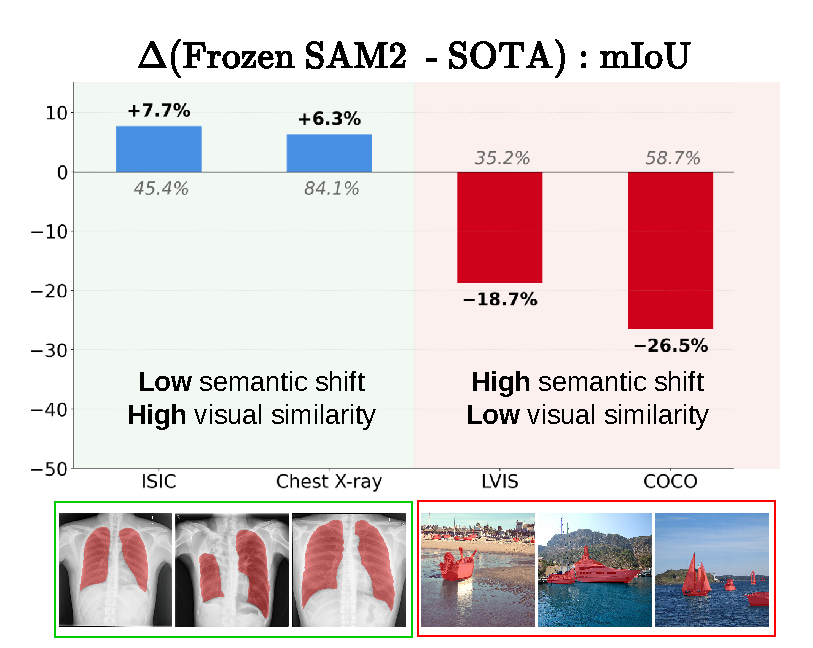
\includegraphics[width=\textwidth]{images/teaser1.pdf}
    \caption{We evaluate frozen \sam{} on few-shot segmentation tasks on four datasets with varying degrees of semantic variability. On datasets \cite{candemir2013lung, codella2019skin} with low semantic shift and high intra-class visual similarity, SAM2 matches or even outperforms state-of-the-art APSeg~\cite{he2024apseg}. However, on more challenging datasets like COCO and LVIS, with high semantic shift (\eg, \textit{cruise ship} vs. \textit{rowboat}), its performance drops significantly, compared with GF-SAM \cite{zhang2024bridge}. The bottom row illustrates examples of ground-truth masks in both scenarios.}
    \label{fig:isic}
\end{minipage}
\hspace{6pt}
\begin{minipage}{0.47\textwidth}
    \centering
    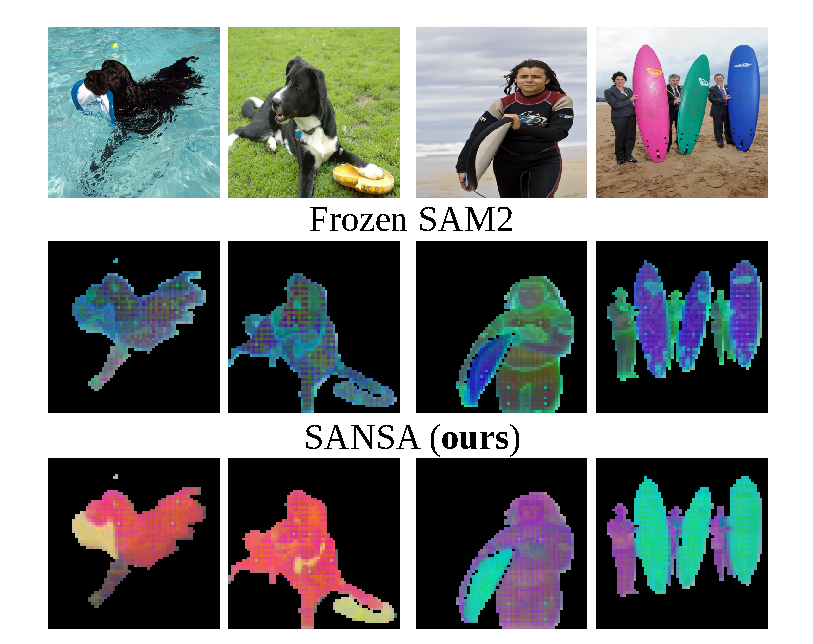
\includegraphics[width=\textwidth]{images/teaser2.pdf}
    %\vspace{0.1cm}
    \caption{We extract \sam{} features from object instances across diverse images and visualize their distribution using the first three principal components of PCA, mapped to RGB channels. The features appear entangled, with clusters mixing across categories, highlighting the lack of a coherent semantic structure in the original feature space. After adapting the feature space with SANSA, well-defined clusters emerge: semantically similar instances group together, forming coherent structures despite intra-class variation in visual appearance.}
    \label{fig:teaser_feat}
\end{minipage}
\vspace{-0.6cm}
%\caption{Overall figure caption describing all three images.}
\end{figure*}

Building on this insight, we introduce \textbf{\ours{}} (\textbf{S}emantically \textbf{A}lig\textbf{N}ed  \textbf{S}egment\textbf{A}nything 2), and show how to expose \sam{} latent semantic structure, repurposing its \texttt{Memory Attention} mechanism to shift from \textit{visual similarity} to \textit{semantic similarity}. The effectiveness of \ours{} is illustrated in \cref{fig:teaser_feat}, where a 3D PCA, computed on \textit{unseen} classes, reveals the emergent semantic organization of our features. 
We complement our method with a novel training objective designed to exploit \sam{} temporal continuity to convert each target image into a \textit{pseudo-annotation} for subsequent frames.

\noindent Our contributions are the following:

\begin{itemize}[noitemsep,topsep=1pt,leftmargin=*]
    \item We are the first to investigate the semantic structure within \sam{}. We show that such semantics can be disentangled through bottleneck transformations, enabling a unified approach that reinterprets few-shot segmentation as the task of tracking semantic concepts across images;
    
    \item We validate \ours{} through extensive experiments, achieving SOTA performance in strict FSS benchmarks while also outperforming generalist approaches in the ‘in-context’ scenario.
    Our experiments reveal that \sam{} encodes coarse-to-fine semantics, from high level concepts (\eg \textit{dog} vs. \textit{cat}, +6.3\% on COCO-20$^i$) to fine-grained distinctions at category-level (\eg \textit{dalmatian} vs. \textit{bulldog}, +8.3\% on LVIS-92$^i$) and part-level (\eg \textit{hand} vs. \textit{arm} +4.6\% on Pascal-Part);
    
    \item By supporting prompts like points, boxes, or scribbles, our approach enables a wide range of downstream task, such as data annotation without the need for costly pixel-level masks. Finally, by exploiting the tight integration of memory attention and mask decoding in \sam{}, we avoid the need for auxiliary models or complex pipelines, setting a new SOTA with a framework more than {3× faster} than competitors, and {4-5× smaller} in parameter count.
\end{itemize}


